\chapter{Introduction}

\section{Introduction}

Welcome to this introduction to SEXTANTE. This text is targeted at those using geospatial algorithms from the SEXTANTE library through the graphical elements also included in the library.

SEXTANTE is integrated into some of the most popular Java desktop GIS, and using it is identical no matter which GIS you are using. If you have a GIS application which incorporates SEXTANTE as its analysis platform, then this manual is for you.

Particular information about SEXTANTE algorithms is not found in this text. The user should refer to the context help system instead.


\section{Basic elements of the SEXTANTE GUI}

There are four basic elements in the SEXTANTE GUI, which are used to run SEXTANTE algorithms for different purposes. Chosing one tool or another will depend on the kind of analysis that is to be performed and the particular characteristics of each user an project.

Depending on the implementation of the GIS application you are using, these elements can be accesed through menu entries (usually under a menu group named ``SEXTANTE'') or a toolbar like the one shown next.

\begin{center}
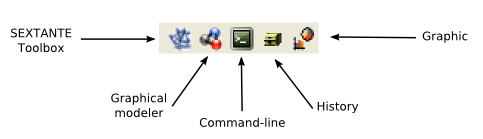
\includegraphics[width=.5\columnwidth]{sextante_objects.png}
\end{center}

\begin{itemize}
	\item The SEXTANTE toolbox. The main element of the SEXTANTE GUI, it is used to execute a single algorithm or run a batch process based on that algorithm.
		\begin{center}
		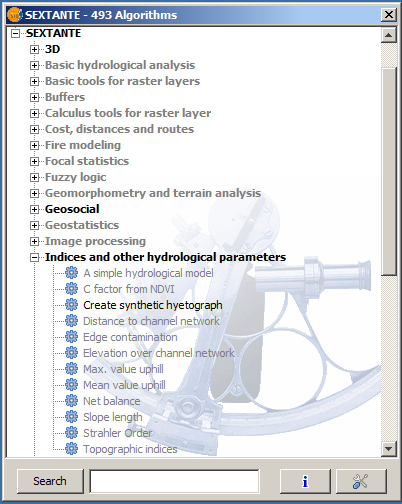
\includegraphics[width=.5\columnwidth]{toolbox.png}
		\end{center}
	\item The SEXTANTE graphical modeler. Several algorithms can be combined graphically using the modeler to define a workflow, creating a single process that involves several sub--processes
		\begin{center}
		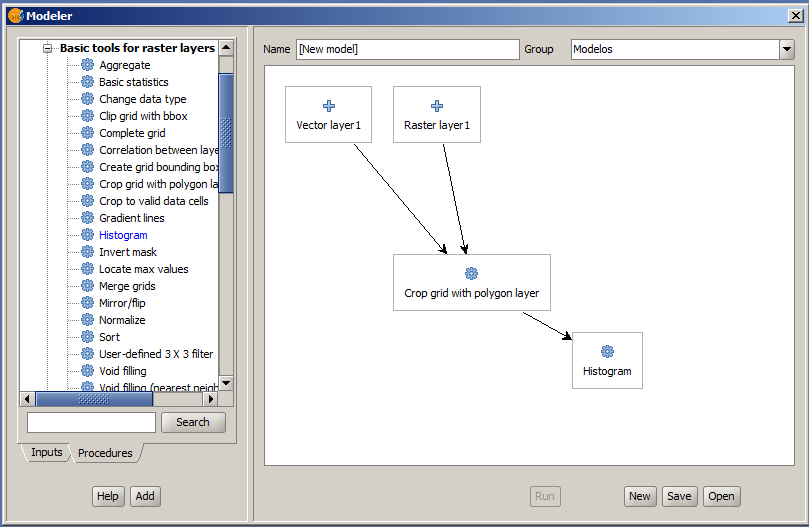
\includegraphics[width=.8\columnwidth]{models.png}
		\end{center}			
	\item The SEXTANTE command--line interface. Advanced users can use this interface to create small scripts and call SEXTANTE algorithms from them
		\begin{center}
		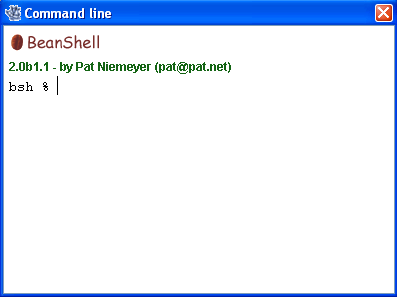
\includegraphics[width=.6\columnwidth]{command_line.png}
		\end{center}
	\item The SEXTANTE history manager. All actions performed using any of the aforementioned elements are stored in a history file and can be later easily reproduced using the history manager
			\begin{center}
			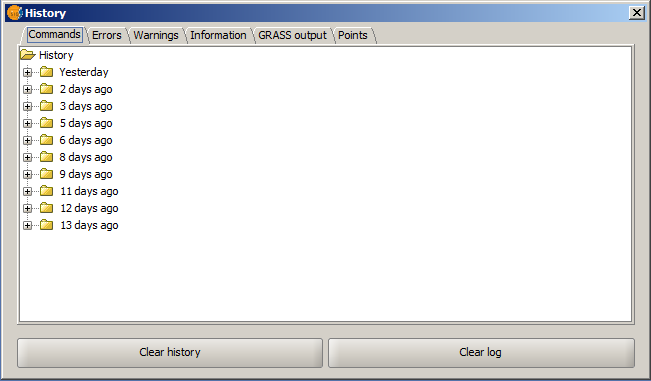
\includegraphics[width=.8\columnwidth]{history.png}
			\end{center}	
\end{itemize}

Along the following chapters we will review each one of this elements in detail.